\chapter{Stockage des boîtes et visualisation}
Trois difficultés majeures apparaissent dans la réalisation du logiciel de visualisation. La première est bien entendu la gestion d'une très grande quantité de boîtes lors de l'affichage. Il est en effet nécessaire d'offrir un accès rapide aux informations des boîtes dans la fenêtre. La seconde est la gestion des filtres sur ces mêmes boîtes. Et le troisième apparait lors du changement des variables étudiées (changement des dimensions visualisées). Dans cette section, nous chercherons d'avantage à apporter une solution pour les problèmes de temps d'accès et de changement de variables. Il est en effet probable que la gestion des filtres soit effectuée par une structure différente.

\section{\'Etude d'une solution possible : le QuadTree}
\paragraph{}Une des solutions qui pourrait permettre une visualisation fluide du pavage tout en répondant au document de spécifications serait de représenter le pavages sous une forme de QuadTree pour deux dimensions ou OcTree pour trois dimensions.
\begin{figure}[htbp]
\centering
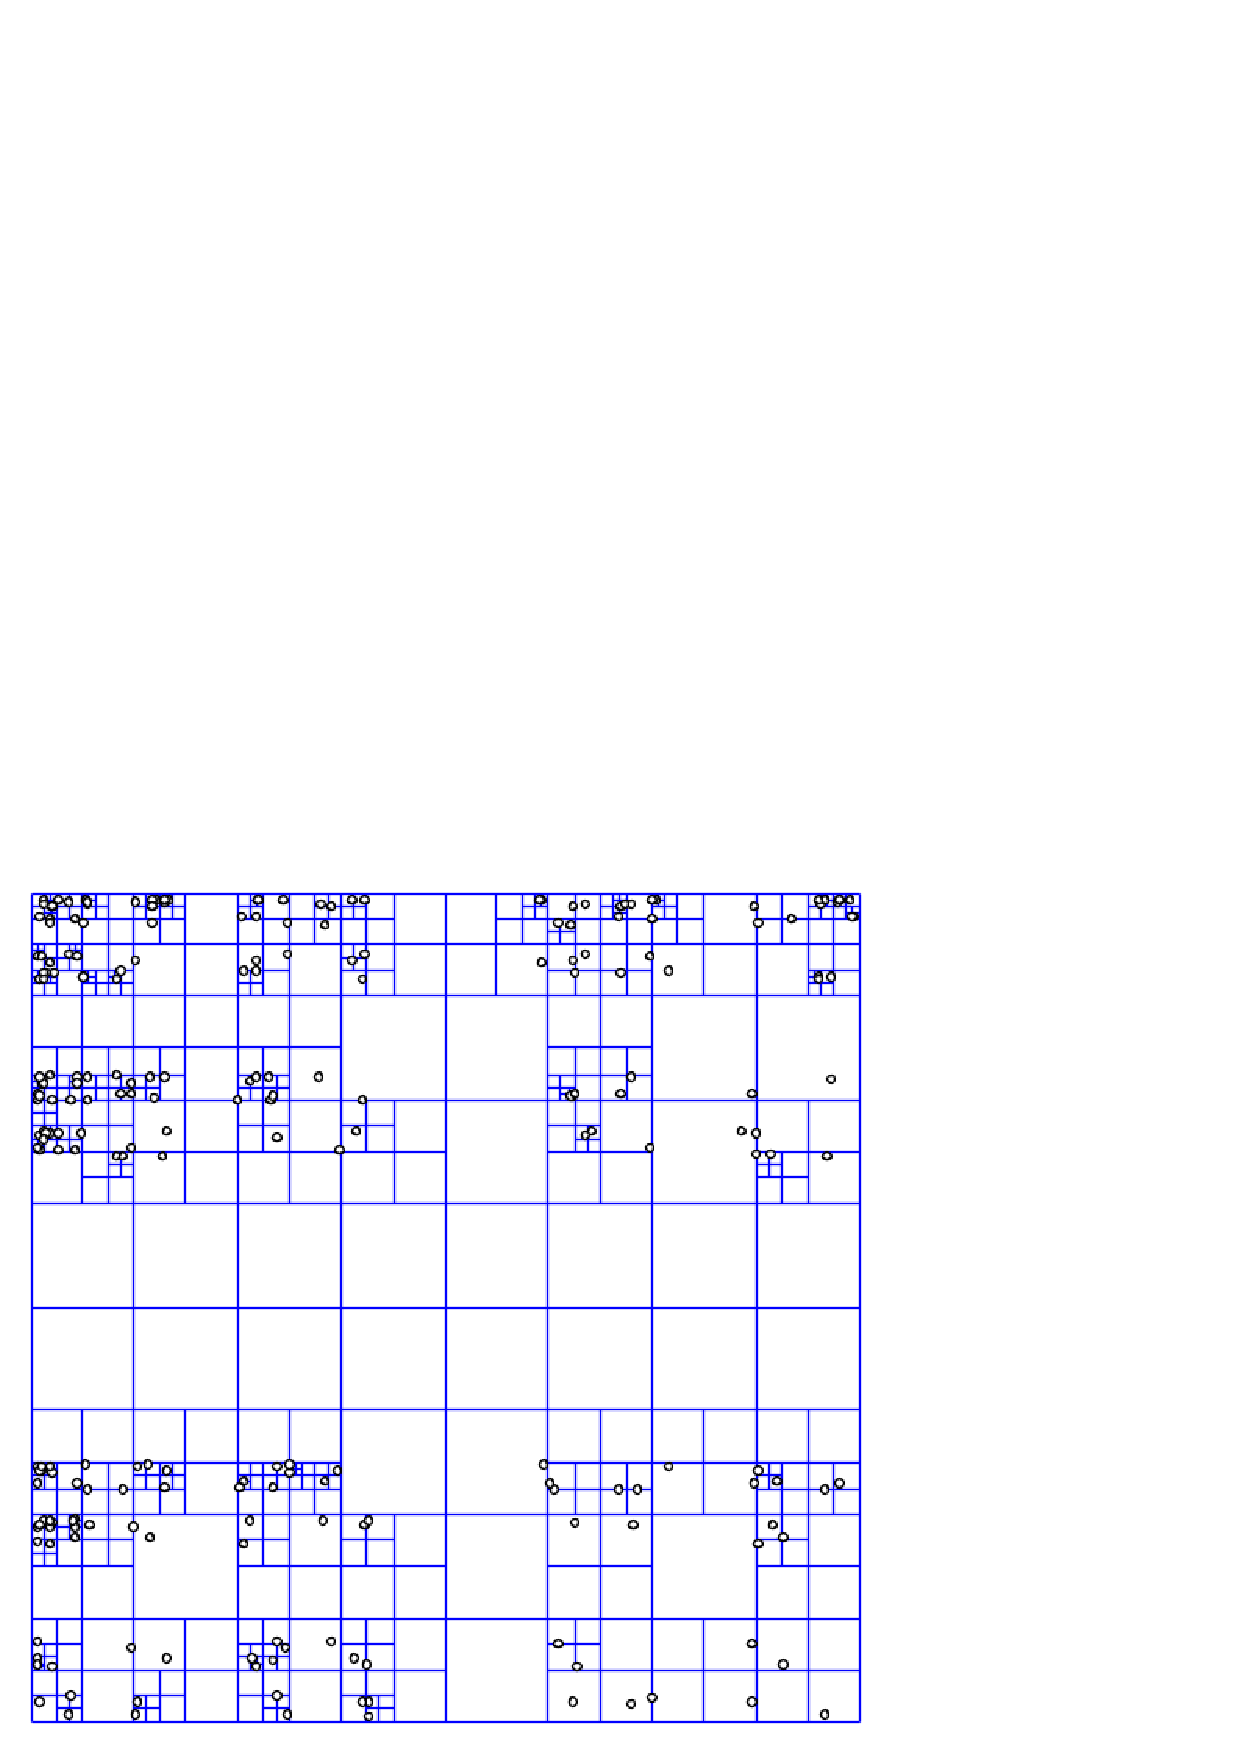
\includegraphics[scale=0.50]{quadtree}
\caption{Représentation d'un quadtree où les données sont des points}
\end{figure}

Le QuadTree consiste à découper récursivement un espace fini en deux dimensions en quatre parties égales. Chacune de ces parties sont stockées dans un nœud. On itère ce mécanisme sur chacun de ces nœuds jusqu'à isoler spatialement les éléments recherchés.

Cette structure pourrait être utilisée pour déterminer la position des boîtes dans l'espace.

\paragraph{}L'algorithme permettant de partitionner est récursif. Dans le cas récursif, l'algorithme divise l'espace en quatre et itère sur chaque sous-espace. Dans le cas d'arrêt on ne subdivise plus. Nous décrivons par la suite l'ensemble des cas de récursions et d'arrêts pour la division d'un espace donné. Les images jointes au texte sont des représentations des différents cas dans lesquels les cadres rouges sont des boîtes solutions et les cadres noirs un espace fourni à l'algorithme. Vous trouverez une classification visuelle dans la table \ref{tab:algo}.
\begin{itemize}
\item Cas d'arrêts : 
\begin{itemize}
\item L'espace fourni est entièrement inclus dans une boîte 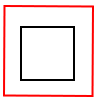
\includegraphics[scale=0.20]{img/QT1}.
\item L'espace fourni contient entièrement une seule boîte 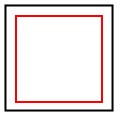
\includegraphics[scale=0.20]{img/QT2}.
\item L'espace fourni contient en partie une seule boîte 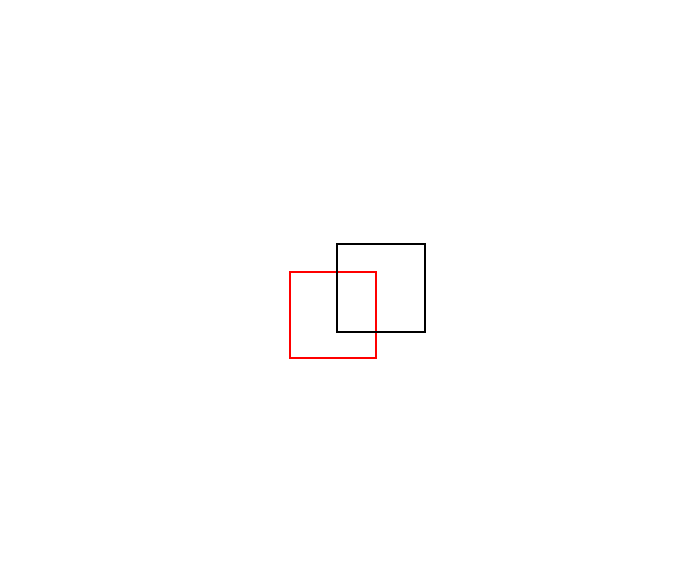
\includegraphics[scale=0.20]{img/QT3}.
\item L'espace fourni n'intersecte aucune boîte 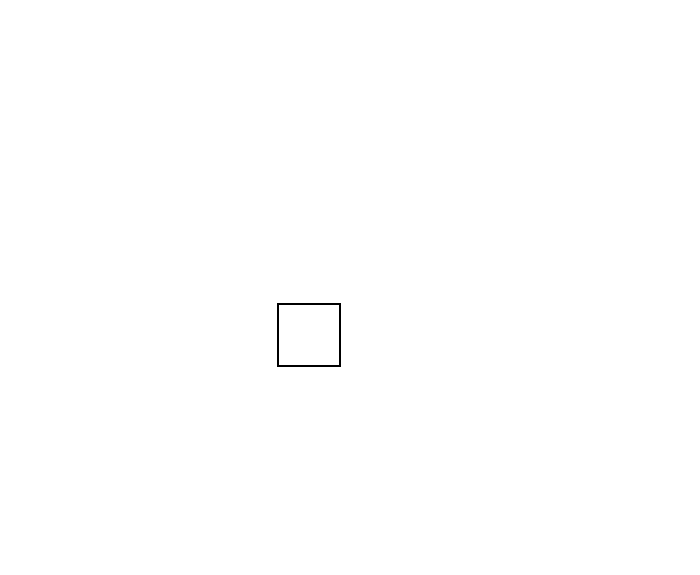
\includegraphics[scale=0.30]{img/QT6}.
\item L'espace fourni ne peux plus être subdivisé car on a fourni une taille minimale pour les espaces.
\end{itemize}
\item cas de récursions :
\begin{itemize}
\item L'espace fourni intersecte plusieurs boîtes 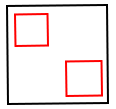
\includegraphics[scale=0.20]{img/QT4} ou encore 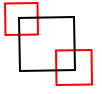
\includegraphics[scale=0.20]{img/QT5}.
\end{itemize}
\end{itemize}

\begin{table}[htbp]
\centering
 \begin{tabular}{|c|cccc|}
  \hline
  Cas de récursion &  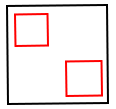
\includegraphics[scale=0.20]{img/QT4}&  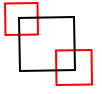
\includegraphics[scale=0.20]{img/QT5}& &\\
  \hline
  Cas d'arrêt&  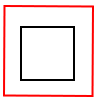
\includegraphics[scale=0.20]{img/QT1}&  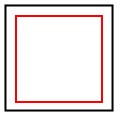
\includegraphics[scale=0.20]{img/QT2}&  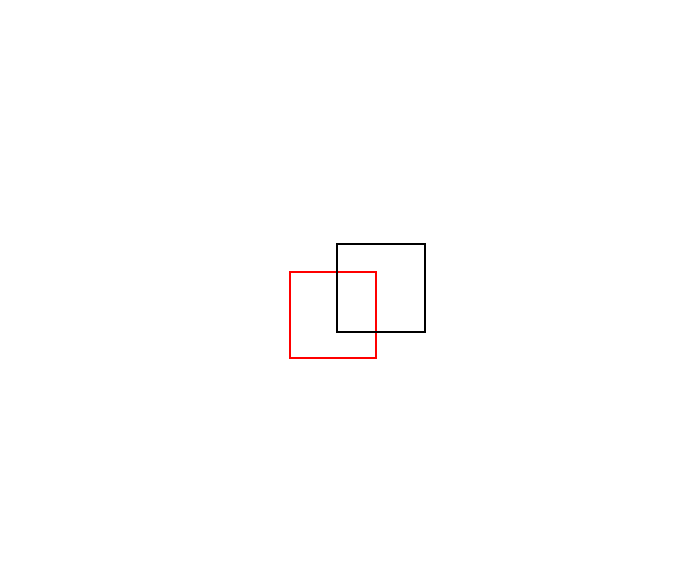
\includegraphics[scale=0.20]{img/QT3}&  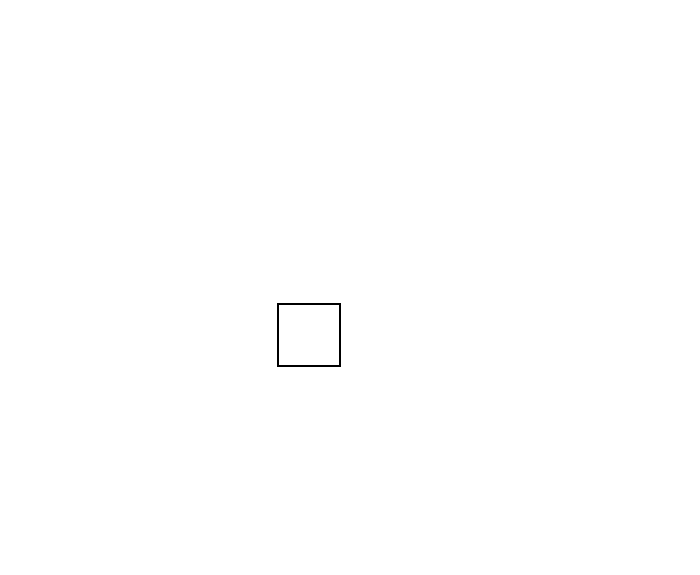
\includegraphics[scale=0.30]{img/QT6}\\
  \hline
 \end{tabular}
 \caption{Classification visuelle des cas d'arrêts et de récursions}
\label{tab:algo}
\end{table}


L'OcTree repose sur le même principe mais étendu à trois dimensions. L'espace est donc découpé en huit parties à chaque fois.

\paragraph{Avantage de cette méthode}Cette structure est particulièrement intéressante pour la visualisation du pavage. En effet pour une fenêtre de visualisation donnée, il est très simple et rapide d'extraire la sous-arborescence correspondante à l'espace visualisé et permet aussi de ne pas afficher les objets trop petits. 

De plus il serait possible de créer une structure reposant sur le même principe que le QuadTree mais étant $k$-dimensionnelle\footnote{$k$ étant la dimension du problème fourni à Realpaver.}. Chaque espace peut alors être potentiellement subdivisé en $2^k$ sous-espaces. Cette structure permettrait d'éviter de recalculer l'arbre à chaque changement de variables de visualisation. On évite par ailleurs le cas de superposition de boîtes pour lequel l'algorithme n'est plus efficace (cf : figure \ref{fig:superpos}).
\begin{figure}[htbp]
\centering
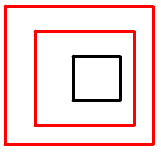
\includegraphics[scale=0.30]{img/QT8}
\caption{Superposition de boîtes}
\label{fig:superpos}
\end{figure}

\paragraph{Inconvénient de cette méthode}Le problème majeur de cette méthode se présente lorsque des boîtes sont côte à côte (cf : figure \ref{fig:frontiere}).
\begin{figure}[htbp]
\centering
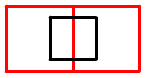
\includegraphics[scale=0.40]{img/QT7}
\caption{Superposition de boîtes 1}
\label{fig:frontiere}
\end{figure}
Dans une telle situation chaque division va entrainé la création d'un espace dans la même configuration. L'algorithme ne s'arrêtera donc pas avant d'avoir atteint la taille minimale d'un espace. Nous nous retrouvons donc avec un grand nombre de boîtes au niveau de ces \og frontières\fg{} (cf : figure \ref{fig:frontiere2}).
\begin{figure}[htbp]
\centering
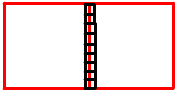
\includegraphics[scale=0.40]{img/QT9}
\caption{Superposition de boîtes 2}
\label{fig:frontiere2}
\end{figure}
Ainsi sachant que la précision maximale par défaut de \emph{Realpaver} est de $10^{-16}$, cela implique qu'il est nécessaire d'au moins égaler cette précision pour l'arbre de visualisation. Ainsi pour une sortie de \emph{Realpaver} contenant un total $l$ de longueurs de \og frontières \fg{}  cumulées et $p$ la précision du modèle, on a un nombre d'espaces à créer supérieur à $\frac{l}{p}$ avec $p$ très petit. Par exemple pour une sortie de \emph{Realpaver} comportant une \og frontière \fg{} de taille $1$, il faudra au moins $10^{16}$ espaces pour la contenir. 

\paragraph{Brève conclusion} Le QuadTree est une structure intéressante pour la visualisation mais si un nœud de l'arbre a un coût en mémoire non nul, alors l'espace mémoire de la structure va exploser. Elle semble donc, pour le moment, inappropriée.

\section{\'Etude d'une seconde solution : le R-tree}
\paragraph{}Bien que le QuadTree soit une structure intéressante pour permettre l'indexation et la recherche de points dans un espace, celui-ci l'est beaucoup moins pour la gestion de données à dimensions non nulles. Le R-tree est une structure proposé en 1984 par Antonin \textsc{Guttman} permettant l'indexation et la recherche d'éléments de dimension $d > 0$ dans $k$ dimensions\cite{Guttman}.

\paragraph{}Le R-tree est une variante équilibré de l'arbre B, sa structure est la suivante :
\begin{itemize}
 \item Un noeud de l'arbre correspond à une boîte non-solution du pavage ( généralement appelé \og page \fg{}).
 \item Chaque boîte peut contenir entre $m$ et $M$ sous-boîtes entièrement incluses. Avec $m\leq \frac{M}{2}$.
 \item Une feuille de l'arbre est une boîte ne contenant que des boîtes solution du pavage.
\end{itemize}

La figure \ref{fig:rtree} donne une bonne idée de l'organisation des R-trees:
\begin{figure}[htbp]
\centering
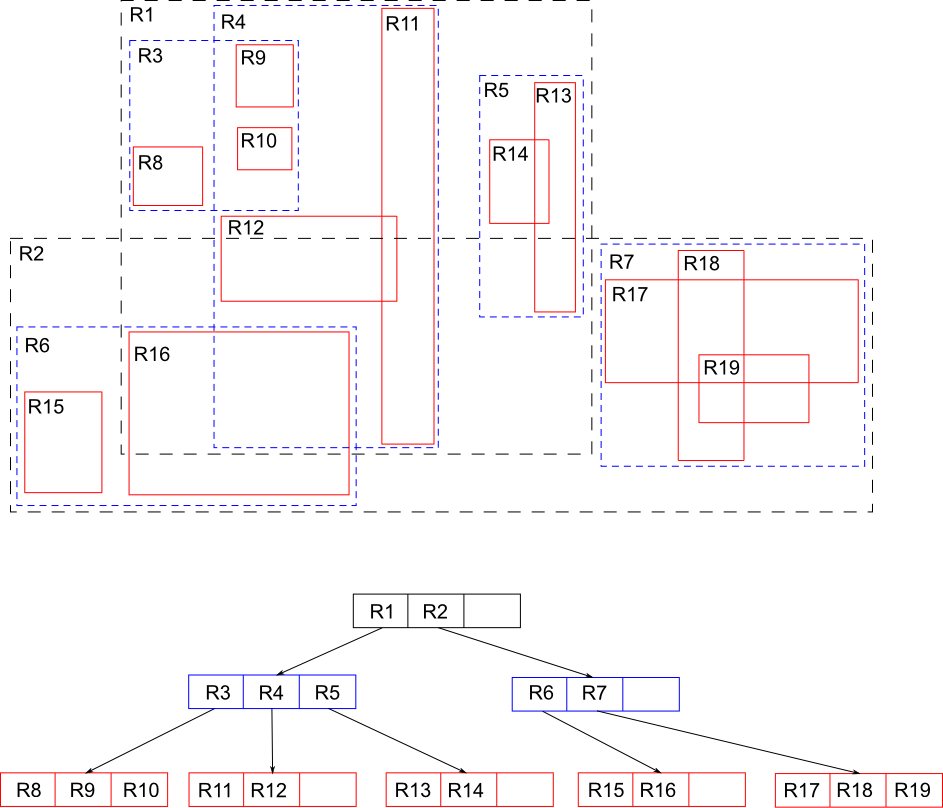
\includegraphics[scale=0.50]{rtree}
\caption{Représentation d'un R-tree\cite{wiki}}
\label{fig:rtree}
\end{figure}

Les algorithmes permettant la recherche et la création du R-tree sont qu'en à eux décrient dans l'article de \textsc{A. Guttman} dans la section \textbf{3. Searching and Updating}\cite{Guttman}.

\paragraph{Avantages et inconvénients du R-tree} Le R-tree est une structure de données spécialement conçue pour la recherche de données à dimensions $d$ pour dans des espaces $k$-dimensionnels. L'arbre a une profondeur maximale $h_{max}$ égale à :
\begin{equation}
 h_{max} = \left\lceil\log_{m} n\right\rceil - 1
\end{equation}
et le nombre de nœuds est au pire égale à :
\begin{equation}
 \sum_{i=1}^{h_{max}}{\left\lceil\frac{n}{m^i}\right\rceil} = \left\lceil\frac{n}{m}\right\rceil + \left\lceil\frac{n}{m^2}\right\rceil + \cdots + 1
\end{equation}

 Bien que ne pouvant garantir de bonnes performances en pire cas\footnote{\og \emph{More than one substree under a node may need to be searched, hence it is not possible to guarantee good worst-case performance.}\fg{}\cite{Guttman}, section \textbf{3.1 Searching}}, le R-tree offre en pratique de bons résultats ; on pourra d'ailleurs se reporter à l'analyse de performances effectuer par A. \textsc{Guttman}\footnote{section \textbf{4. Performance}\cite{Guttman}}. Cependant il existe aujourd'hui de nombreuses variantes du R-tree ( R*tree, Hilbert R-tree, etc\dots{} ), on pourra donc, pour une analyse plus générale des différentes implémentations, préférer \og\emph{R-trees : Theory and Applications} \fg{}\cite{poulos}.